\documentclass{article}
\usepackage[margin=1in]{geometry}
\usepackage{amsmath}
\usepackage{amssymb}
\usepackage{amsthm}
\usepackage{bm}
\usepackage{hyperref}
\usepackage{graphicx}
\usepackage{caption}
\usepackage{listings}
\usepackage{xcolor}
\usepackage{float}
\usepackage{booktabs}
\usepackage{longtable}
\usepackage{multirow}
\usepackage{placeins}
\graphicspath{{figures/}}

% Code style
\lstdefinestyle{code}{
  basicstyle=\ttfamily\small,
  numbers=left,
  numberstyle=\tiny,
  numbersep=8pt,
  keywordstyle=\color{blue},
  commentstyle=\color{teal!70!black},
  stringstyle=\color{orange!70!black},
  showstringspaces=false,
  breaklines=true,
  frame=single,
  framerule=0.3pt,
  rulecolor=\color{black!15}
}
\lstset{style=code}

\title{Multi-Agent Systems: Architecture, Frameworks, Coordination, and Applications}
\author{}
\date{\today}

\begin{document}
\maketitle

\section{Agent Architecture: Planner, Executor, Memory, Tooling}
\subsection{Layered anatomy}
Modern multi-agent setups adopt a layered decomposition where planners transform goals into action plans, executors carry out atomic steps, memory modules retain context, and tooling bridges external systems. Figure~\ref{fig:multi_agent_architecture_en} summarizes the signal flow and feedback paths.
\begin{figure}[H]
  \centering
  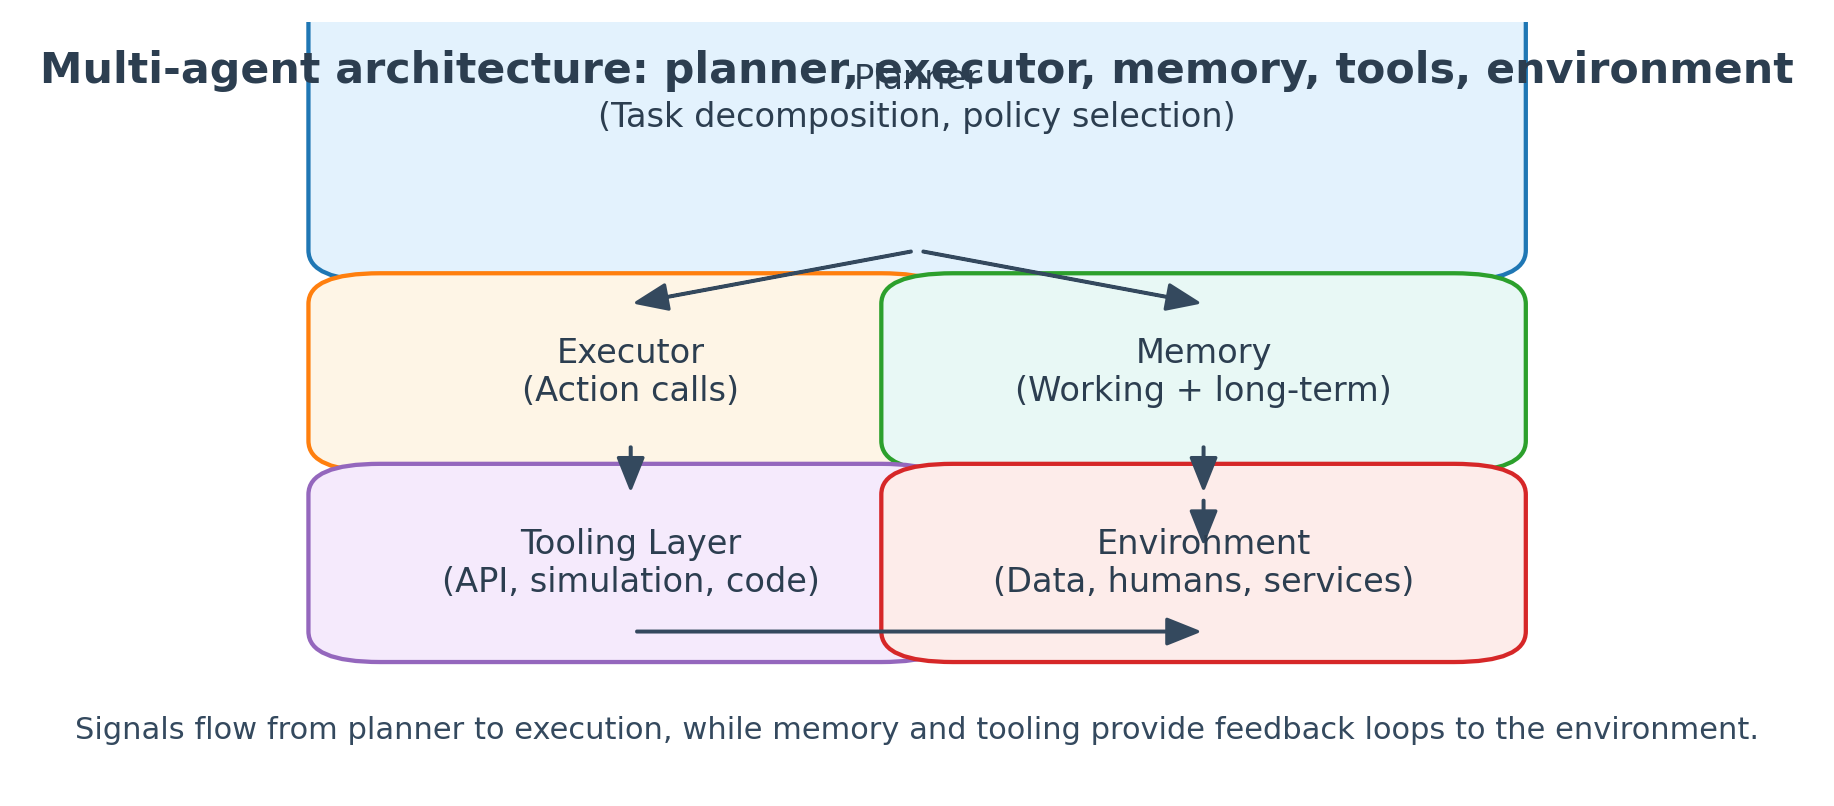
\includegraphics[width=0.95\textwidth]{multi_agent_architecture.png}
  \caption{Multi-agent architecture spanning planner, executor, memory, tooling, and environment interfaces.}
  \label{fig:multi_agent_architecture_en}
\end{figure}

\subsection{Module responsibilities}
\begin{itemize}
  \item \textbf{Planner:} Ingest objectives, constraints, and memory snapshots to output decomposed tasks or policies; leverage tree search, PDDL planning, or reinforcement critics.
  \item \textbf{Executor:} Perform actions (API calls, code execution, simulations) and report observations; often follows the ReAct format (Thought, Action, Observation).
  \item \textbf{Memory:} Combine working memory (conversation state, intermediate artifacts) with long-term knowledge bases (vector stores, knowledge graphs, logs).
  \item \textbf{Tooling Layer:} Provide declarative interfaces to verified tools (retrievers, shells, IDEs, cloud APIs) with rate limiting and access auditing.
  \item \textbf{Environment:} Real-world systems, humans, and data services that respond to actions and impose constraints.
\end{itemize}

\subsection{Design guidelines}
\begin{itemize}
  \item Close the loop between planner and executor through explicit feedback signals to adapt plans dynamically.
  \item Gate tool usage with sandboxing, allow-lists, and guard agents to mitigate unsafe or expensive operations.
  \item Support multimodal inputs/outputs by wrapping perception modules (vision, speech) as tools and writing embeddings into memory.
\end{itemize}

\section{LangChain, CrewAI, and AutoGPT Frameworks}
\subsection{Ecosystem comparison}
\begin{longtable}{p{3.2cm}p{4.5cm}p{6cm}}
\toprule
Framework & Highlights & Ideal scenarios \\
\midrule
LangChain & Modular chains, AgentExecutor APIs, rich memory/tools ecosystem, strong community & Rapid prototyping, workflow automation, enterprise integration \\
CrewAI & Multi-agent team orchestration with role assignments, task boards, sync/async scheduling & Collaborative content creation, knowledge ops, research pods \\
AutoGPT & Autonomous goal pursuit, persistent memory, plugin tooling, filesystem integration & Exploratory research, long-running automation (requires strict safeguards) \\
\bottomrule
\end{longtable}

\subsection{LangChain AgentExecutor example}
\begin{lstlisting}[language=Python,caption={Planner-executor agent implemented with LangChain}]
from langchain.agents import initialize_agent, AgentType, Tool
from langchain.chat_models import ChatOpenAI
from langchain.memory import ConversationBufferMemory
import requests

def fetch_latest(query: str) -> str:
    response = requests.get(
        "https://api.serpapi.com/search",
        params={"q": query, "api_key": "KEY"},
        timeout=10,
    )
    return response.json().get("organic_results", [])

tools = [
    Tool(
        name="web_search",
        func=lambda q: str(fetch_latest(q)[:3]),
        description="Useful for retrieving up-to-date information from the open web."
    )
]

llm = ChatOpenAI(model="gpt-4o-mini", temperature=0)
memory = ConversationBufferMemory(memory_key="chat_history", return_messages=True)

agent = initialize_agent(
    tools=tools,
    llm=llm,
    agent=AgentType.CONVERSATIONAL_REACT_DESCRIPTION,
    memory=memory,
    verbose=True,
)

answer = agent.run("Generate a research brief on deep geothermal inversion techniques.")
print(answer)
\end{lstlisting}

\subsection{CrewAI collaboration}
CrewAI models teams of specialized agents:
\begin{itemize}
  \item Define roles (Researcher, Author, Reviewer) each with tools and memory scopes;
  \item Employ synchronous pipelines for deterministic flows, asynchronous execution for throughput;
  \item Track progress with task boards, enabling human oversight and reruns.
\end{itemize}

\subsection{AutoGPT deployment considerations}
\begin{itemize}
  \item Restrict command execution to sandboxed directories and whitelisted shells;
  \item Use supervisor or guard agents to vet commands before execution;
  \item Rotate memory stores (vector DB, local files) and implement retention policies.
\end{itemize}

\section{Autonomous Planning and Multi-Agent Coordination}
\subsection{Collaboration topology}
Figure~\ref{fig:agent_collaboration_en} highlights a tri-agent collaboration pattern—research, coding, and analysis—coordinated by an orchestrator and shared memory hub.
\begin{figure}[H]
  \centering
  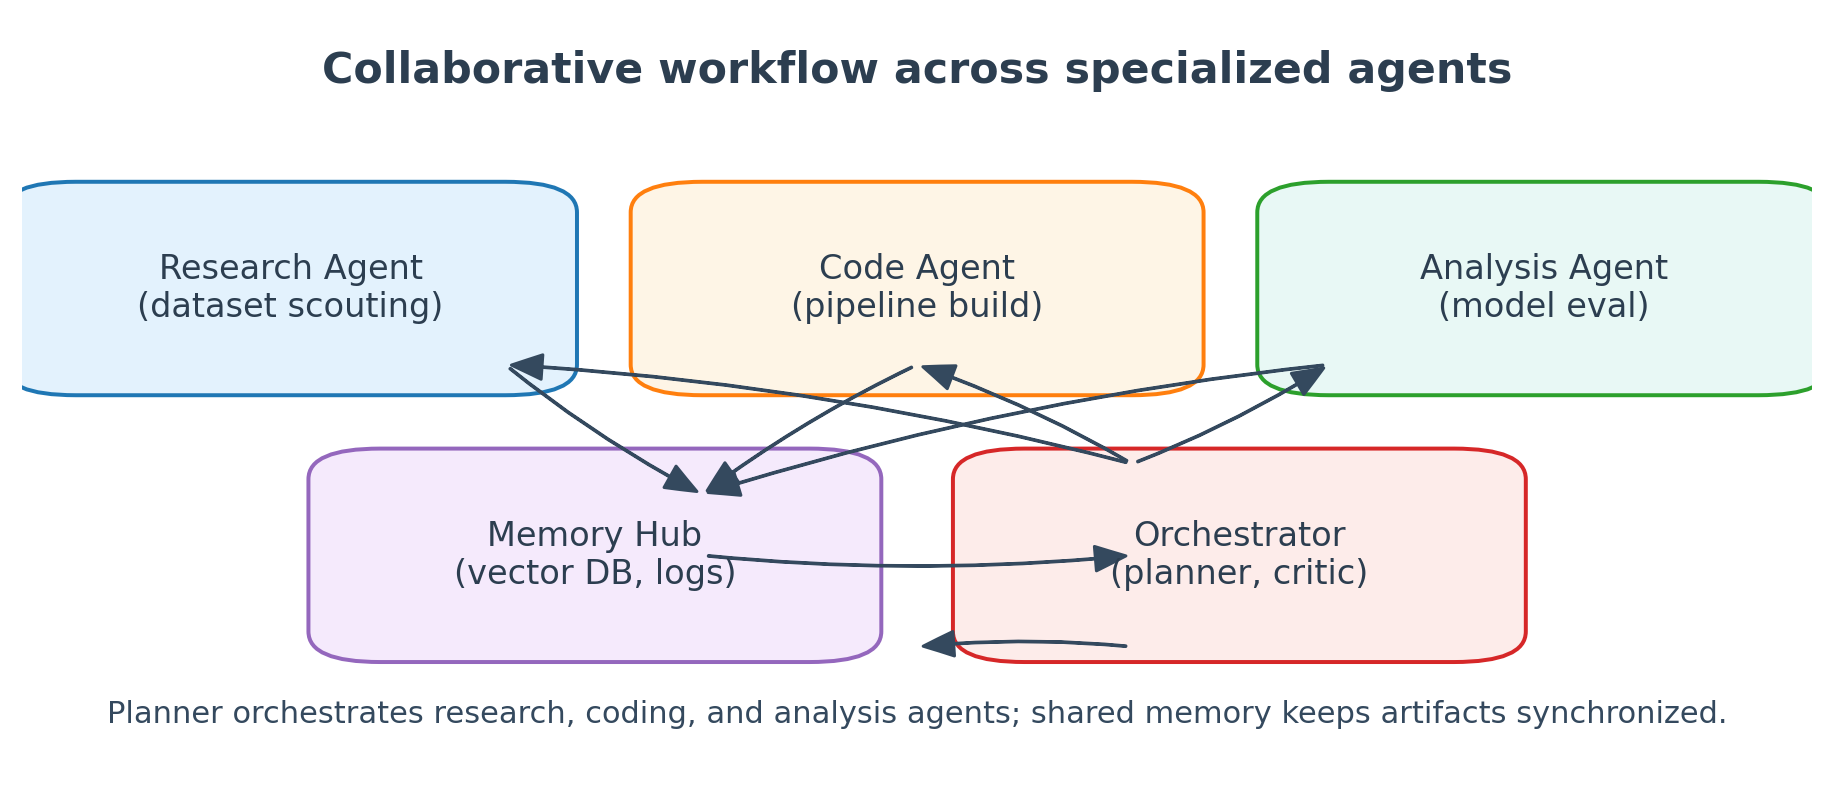
\includegraphics[width=0.95\textwidth]{agent_collaboration.png}
  \caption{Collaborative workflow with specialized agents, shared memory, and orchestration.}
  \label{fig:agent_collaboration_en}
\end{figure}

\subsection{Planning strategies}
\begin{itemize}
  \item \textbf{Hierarchical planning:} High-level planner sets milestones; sub-planners derive step-by-step action lists, optionally with HTN templates.
  \item \textbf{Adaptive scheduling:} Prioritize tasks based on reward signals, confidence scores, or resource budgets; reschedule on failure.
  \item \textbf{Consensus mechanisms:} Debate, critique, or voting agents evaluate outputs to reduce hallucinations and confirm correctness.
  \item \textbf{Conflict management:} Apply locking, transactions, or optimistic concurrency for shared resources and document edits.
\end{itemize}

\subsection{Coordination patterns}
\begin{itemize}
  \item Pipeline: agents operate sequentially, suitable for fixed processes (report assembly).
  \item Blackboard: agents post intermediate artifacts to a shared board, enabling opportunistic collaboration.
  \item Market: agents bid for tasks via utility scores, aligning resource usage with value.
  \item Alliance: agents form sub-teams to tackle complex subproblems, sharing internal state privately.
\end{itemize}

\subsection{Metrics and observability}
\begin{longtable}{p{3cm}p{3cm}p{4cm}p{4cm}}
\toprule
Category & Metrics & Focus & Instrumentation \\
\midrule
Efficiency & Task latency, throughput, utilization & Scheduling performance & Prometheus, OpenTelemetry \\
Quality & Human ratings, automated graders, benchmark scores & Output accuracy and clarity & GPT judges, golden datasets \\
Collaboration & Communication volume, conflict rate, success ratio & Coordination overhead & Log analytics, replay systems \\
Safety & Denied actions, policy violations, rollback count & Risk management & Audit trails, guardrail dashboards \\
\bottomrule
\end{longtable}

\section{Applications: Research, Code Generation, Geophysical Interpretation}
\subsection{Scientific research assistants}
\begin{itemize}
  \item \textbf{Literature review:} Research agent queries academic APIs, aggregates abstracts into a vector memory with metadata tags.
  \item \textbf{Experiment design:} Code agent drafts scripts, container specs, and configuration files; execution logs are persisted for reproducibility.
  \item \textbf{Manuscript drafting:} Writing agent composes sections using memory summaries, reviewer agent checks citations and style compliance.
\end{itemize}

\subsection{Software engineering copilots}
\begin{itemize}
  \item \textbf{Requirement analysis:} Planner breaks down epics into tickets; code agent commits patches and launches unit tests.
  \item \textbf{Security gating:} Security agent runs static analyzers, fuzzers, and policy checks; guard agent enforces dependency policies.
  \item \textbf{DevOps integration:} Deployment agent interacts with CI/CD pipelines, handles rollback procedures, and updates observability dashboards.
\end{itemize}

\subsection{Geophysical interpretation}
\begin{itemize}
  \item \textbf{Data assimilation:} Data agent interfaces with seismic or magnetotelluric databases, performs denoising and feature extraction.
  \item \textbf{Inversion modeling:} Simulation agent submits runs to HPC clusters, tracks convergence, and stores volumetric outputs.
  \item \textbf{Interpretation:} Analyst agent summarizes subsurface structures, quantifies uncertainty, and compares against historical wells.
  \item \textbf{Human oversight:} Subject-matter experts inspect dashboards, annotate anomalies, and feed adjustments back into memory.
\end{itemize}

\section*{Operational recommendations}
\begin{itemize}
  \item Define structured communication contracts (JSON schemas, protocol buffers) to ensure agents interoperate safely.
  \item Introduce governance loops—human approval gates, policy engines, red teaming—to maintain reliability.
  \item Centralize logging and telemetry for traceability, latency analysis, and incident response.
  \item Stress-test multi-agent scenarios with adversarial prompts before production rollout to surface failure modes.
\end{itemize}

\section*{Further reading}
\begin{itemize}
  \item Wang et al. ``Voyager: An Open-Ended Embodied Agent with Large Language Models.'' arXiv, 2023.
  \item Shinn et al. ``Reflexion: Language Agents with Verbal Reinforcement Learning.'' NeurIPS, 2023.
  \item Park et al. ``Generative Agents: Interactive Simulacra of Human Behavior.'' SIGGRAPH, 2023.
  \item Qian et al. ``AutoGen: Enabling Next-Gen LLM Applications via Multi-Agent Conversations.'' Microsoft Research, 2023.
  \item Arora et al. ``CrewAI: Orchestrating Collaborative AI Workers.'' arXiv, 2024.
\end{itemize}

\end{document}

